\documentclass[11pt,a4paper]{article}

\usepackage{main}
\usepackage{cours}

\renewcommand{\typedocument}{Document}
\renewcommand{\classe}{5e}
\renewcommand{\titre}{Electricité et sécurité}

\begin{document}

\creertitre{Activité : Sécurité et électricité}

Les effets du courant électrique dépendent de divers facteurs : état de santé, âge, durée
de l’électrisation, conditions d’humidité et surtout de la valeur de la tension électrique.

En dessous de 24 V, il n’y a pas de dangers, c’est la tension de sécurité. A la maison, la tension d’usage est de 230 V.

\vspace{4pt}

\begin{center}
\begin{tabular}{|c|c|c|c|}
\hline
\rowcolor{gray!30}
Tension & Peau sèche & Peau humide & Peau mouillée \\
\hline
30 V & Picotements & Contractions involontaires & Paralysie respiratoire \\
\hline
70 V & Contractions involontaires & Tétanisation des muscles & Mort \\
\hline
230 V & Paralysie respiratoire & Mort & Mort \\
\hline
\end{tabular}
\end{center}

Les deux parties d'une prise électrique sont la borne active (phase) et la borne passive (neutre). On peut s’électriser ou s’électrocuter par contact direct ou indirect entre les deux bornes
ou la borne active et la Terre.

\begin{center}
    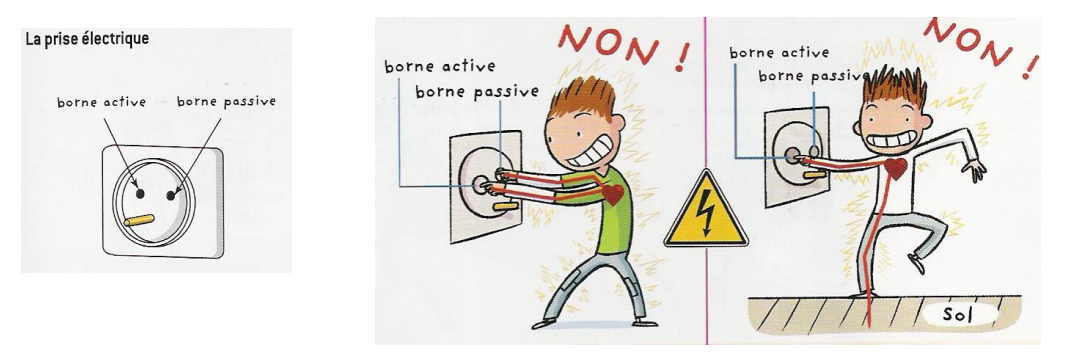
\includegraphics[width=15cm]{images/electrisation.png}
\end{center}

Quelques consignes de sécurité :
\begin{itemize}
    \item Ne pas toucher une borne de prise, que ce soit à mains nues ou à l’aide d’un objet
métallique.
    \item Ne pas utiliser d’appareil électrique dans un environnement humide (salle de bains).
    \item Ne pas bricoler un appareil sans l’avoir d’abord débranché.

\end{itemize}

\vspace{4pt}

\textbf{Questions}

\begin{enumerate}
    \item Quelle est la différence entre électrocution et électrisation ?
    \item A partir de quelle tension il y a-t-il risque d’électrocution ?
    \item Quelle tension ne faut-il pas dépasser pour ne pas avoir de danger ?
    \item Est-ce qu’il peut y avoir un danger avec les appareils ménagers ?
    \item Est-ce qu’il y a un danger avec les générateurs utilisés en classe ?
    \item Dans quels cas peut-on s’électriser ou s’électrocuter avec une prise électrique ?
    \item Quels sont les précautions à prendre pour éviter une électrisation ?
    \item Pourquoi ne faut-il pas toucher une personne qui s’électrise ?
\end{enumerate}

\end{document}

